%\begin{filecontents*}{example.eps}
%!PS-Adobe-3.0 EPSF-3.0
%%BoundingBox: 19 19 221 221
%%CreationDate: Mon Sep 29 1997
%%Creator: programmed by hand (JK)
%%EndComments

%\end{filecontents*}
%
%\documentclass{svjour3}                     % onecolumn (standard format)
%\documentclass[smallcondensed]{svjour3}     % onecolumn (ditto)
\documentclass[12pt,oneside,a4paper]{article}  

\usepackage{apacite}
\usepackage{appendix}
\usepackage{amsmath}
\usepackage{amsthm}
% for ASY interactive 3d figure
\usepackage[inline]{asymptote}
\usepackage{amssymb} % for approx greater than
\usepackage{caption}
\usepackage{placeins} % for \FloatBarrier
\usepackage{graphicx}
\usepackage{subcaption}
\usepackage{longtable}
\usepackage{setspace}
\usepackage{booktabs}
\usepackage{tabularx}
\usepackage{xcolor,colortbl}
\usepackage{chngpage}
\usepackage{natbib}
\bibpunct{(}{)}{,}{a}{}{;} 
\usepackage{url}
\usepackage{nth}
\usepackage{authblk}
\usepackage[most]{tcolorbox}
\usepackage[normalem]{ulem}
\usepackage{amsfonts}

% columns for longtable
%\usepackage{arydshln} % Dashed lines in matrices

\usepackage[margin=1in]{geometry}
%\doublespacing % for review

% line numbers to make review easier
%\usepackage{lineno}
%\linenumbers

%\usepackage{soul}% for \st{}

%%%%%%%%%%%%%%%%%%%%%%%%%%%%%%%%%%%%%%%%%%%%%%%%%%%%%%%%%%%%%%%%%%%%%%%%%%%%%%
% for section 4 math environments
%\theoremstyle{definition}
%\newtheorem{definition}{Definition}[section]
%\newtheorem{theorem}{Theorem}[section]
%\newtheorem{proposition}{Proposition}[section]
%\newtheorem{corollary}{Corollary}[proposition]
%\newtheorem{remark}{Remark}[section]
%


%\newcommand\ackn[1]{%
%  \begingroup
%  \renewcommand\thefootnote{}\footnote{#1}%
%  \addtocounter{footnote}{-1}%
%  \endgroup
%}

%\renewcommand\Affilfont{\small}
\newcommand{\absdiv}[1]{%
  \par\addvspace{.5\baselineskip}% adjust to suit
  \noindent\textbf{#1}\quad\ignorespaces
}

%\defcitealias{HMD}{HMD 2016}

% junk for longtable caption
%\AtBeginEnvironment{longtable}{\linespread{1}\selectfont}
%\setlength{\LTcapwidth}{\linewidth}

% sort van Raalte properly
% #1: sorting key, #2: prefix for citation, #3: prefix for bibliography
%\DeclareRobustCommand{\VAN}[3]{#2} % set up for citation
%\newcommand{\tc}{\quad\quad\text{,}}
%\newcommand{\tp}{\quad\quad\text{.}}
%%%%%%%%%%%%%%%%%%%%%%%%%%%%%%%
\begin{document}


\title{A note on independant time measures}

%\author{Tim Riffe \and Neil Mehta \and Daniel Schneider \and Mikko Myrskyl\"a}
\author[1]{Tim Riffe\thanks{riffe@demogr.mpg.de}}
\author[2]{Joel Cohen}


\affil[1]{Max-Planck-Institute for Demographic Research}
\affil[2]{The Rockefeller University}


%\authorrunning{Short form of author list} % if too long for running head

\maketitle

\vspace{-2em}
\begin{abstract}
\absdiv{Background} There are countless Lexis-like relationships between
linearly dependant time measures, and these can be combined into higher-order
Lexis identities with dense linear interdependencies. One such relationship is
the demographic time identity between age, period, cohort, time to death, length of life, and time of death. Certain subsets of time measures in this
and other higher order identities consist in time measures that are independant
of one another.
\absdiv{Objective} We aim to describe the relationship between
independent time measures and the identities within which they are nested, with
special attention to the demographic time identity and its three independant
time dyads. We also aim to determine whether data structured on such time dyads
might be useful in demographic research.
\absdiv{Data and Methods} We illustrate concepts visually based on data from the
Colonial Qu\'{e}bec Population Register and from the US Health and Retirement study.
\absdiv{Results}  We show that the Cartesian mappings of independant time dyads form a redundant mapping of the same demographic timespace. These add three previously undescribed demographic perspectives to the four Lexis-like perspectives, four a total of seven proposed standard perspectives. 
\absdiv{Conclusions} We show independant sets of time measures to be consistent
with the temporal identities within which they are nested. We demonstrate that
these perspectives can be useful for pattern detection and characterization
in demographic research.
\end{abstract}

\textcolor{red}{This isn't even a first draft! Literally it contains copied and
pasted email conversations at this point. It needs a deep revision before even
becoming a manuscript stub. So please read w caution.}

\section{Data}
We illustrate concepts using two data sources: the \emph{le registre de la
population du Qu\'{e}bec ancien} (RPQA) \citep{desjardins1998}, and RAND version
P of the United States Health and Retirement Study (HRS) \citep{HRS, RAND}. The
RPQA data are used to illustrate perspectives on population structure,
whereas the HRS data are used to illustrate how independant time perspectives
relate can be used to take cross-sections of phenomena with multiple time
dimensions.

\subsection{RPQA}
[Provide a minimal description of RPQA data here, as it may be unfamiliar.]

\subsection{HRS} 
We select a single phenomenon to visualize based on information in the HRS. We
follow the data smoothing steps described by \citet{riffe2017hle} to prepare the
data, and summarize these here.
[write description of data prep here. HRS data likely familiar]

\section{Geometric relationships}
The demographic time identity can be represented as a tetrahedral graph and it
therefore maps to the edges of a tetrahedron.
When extended into three dimensions, the tetrahedron tesselates with octahedra in a 2:1
ratio. In its original description \citep{riffe2017demographictime}, neither
independant pairs of time measures nor the significance of octahedra in this
geometric construct were considered. Figure~\ref{fig:tet}
shows the tetragedral graph of the demographic time identity between age
(A), period (P), cohort (C), time to death (T), death cohort (D), and length
of life (L). Independant dyads are those that do not share any vertex in the
graph, and these appear already as perpendicular but disjoint in the present
graph representation: CT, LP, and AD.

\begin{figure}[h!]
\centering
\caption{Tetrahedral graph of demographic time hexad identity, with edges
labelled by the six time indices. Reproduced from 
\citet{riffe2017demographictime}.}
\label{fig:tet}
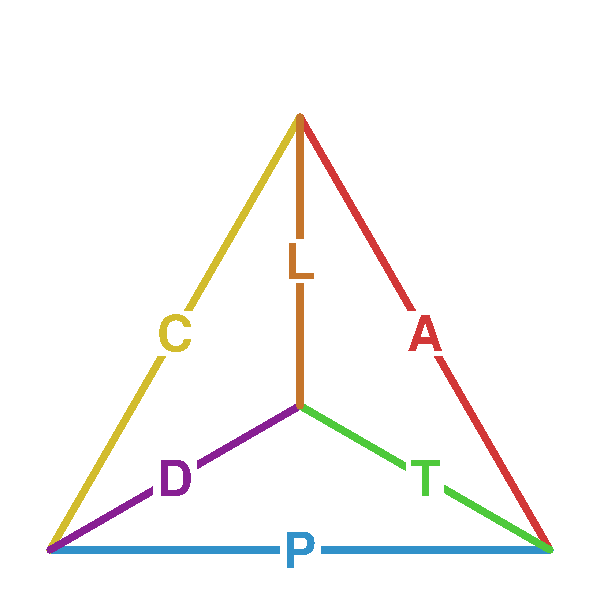
\includegraphics[width=4in]{Figures/TetraHedronEdgesOnly.pdf}%
\end{figure}

Any arbitrary pair of quantitative variables can define the axes of a standard Cartesian plane. When
Cartesian axes are defined by two independant time measures, the resultant plane
is already an isometric projection. However, planes of this kind can also
represent cross-sections of the same 3d demographic timespace previously defined \citep{riffe2017demographictime}.
The independant dyads can also be conceived of as \emph{axes of view} on the
demographic time space.

\subsection{View axes}
An angle of view directly at any of the four faces of the demographic
time tetrahedron reveals the plane-perspective of a
Lexis-like identities. In other words, the viewing axis is set as
\emph{normal} to one of the faces of the tetrahedron. Interactive
figure~\ref{fig:viewaxes} may help visualize the notion of viewing axes--- the
view on a plane is orthogonal if an axis line is reduced to appear as a point in
the centroid of the tetrahedron. The view axes of the four triad identities map
to the four medians (axes of 3-fold symmetry) of the tetrahedron, depicted in
Figure~\ref{fig:depviewaxes} with cyan colored lines.
Independant dyad planes are revealed when the viewing angle is such that the midpoints of opposite tetrahedral edges are aligned. There are three pairs of
opposite edges (LP, TC, AD), and therefore three viewing angles of this kind,
which map to the bimedians of the tetrahedron (axes of 2-fold symmetry),
depicted in Figure~\ref{fig:indepviewaxes} with magenta lines.

\begin{figure}
\begin{subfigure}{.48\textwidth}
\begin{asy}
// DepViewAxes produced by rgl
settings.prc = true;
size(3inches, 3inches);
import graph3;
currentprojection = orthographic(0, -3.101144, 1.128724, up = (0, 0.3420201, 0.9396926));
defaultpen(fontsize(14));
ticklabel RGLstrings(real[] at, string[] label)
{
  return new string(real x) {
    int i = search(at, x);
    if (i < 0) return "";
    else return label[i];
  };
}

ticklabel RGLScale(real s)
{
  return new string(real x) {return format(s*x);};
}
currentlight = light(ambient=new pen[] {rgb(1,1,1)},
diffuse = new pen[] {rgb(1,1,1)},
specular = new pen[] {rgb(1,1,1)},
position = new triple[] {(0,0,1)},
viewport = true);
currentpen += linewidth(4);
currentpen = colorless(currentpen) + rgb(0.1921569, 0.5686275, 0.7882353);
draw((0.4985029, 0, -0.1762474)
--(-0.2492514, 0.4317162, -0.1762474)
);
label("P", position = (-0.002741766, 0.3181748, -0.1938721), align = (0,0));
currentpen = colorless(currentpen) + rgb(0.8235294, 0.7372549, 0.1764706);
draw((0.4985029, 0, -0.1762474)
--(-0.2492514, -0.4317162, -0.1762474)
);
label("C", position = (-0.002741766, -0.3181748, -0.1938721), align = (0,0));
currentpen = colorless(currentpen) + rgb(0.5333334, 0.1215686, 0.5764706);
draw((0.4985029, 0, -0.1762474)
--(0, 0, 0.5287422)
);
label("D", position = (0.1809565, 0, 0.3257052), align = (0,0));
currentpen = colorless(currentpen) + rgb(0.8235294, 0.2156863, 0.2156863);
draw((-0.2492514, 0.4317162, -0.1762474)
--(-0.2492514, -0.4317162, -0.1762474)
);
label("A", position = (-0.2741766, -0.1614619, -0.1938721), align = (0,0));
currentpen = colorless(currentpen) + rgb(0.3058824, 0.7882353, 0.2313726);
draw((-0.2492514, 0.4317162, -0.1762474)
--(0, 0, 0.5287422)
);
label("T", position = (-0.09047827, 0.156713, 0.3257052), align = (0,0));
currentpen = colorless(currentpen) + rgb(0.772549, 0.4588235, 0.1686275);
draw((-0.2492514, -0.4317162, -0.1762474)
--(0, 0, 0.5287422)
);
label("L", position = (-0.09047827, -0.156713, 0.3257052), align = (0,0));
currentpen += linewidth(2);
currentpen = colorless(currentpen) + rgb(0, 1, 1);
draw((0, 0, 0.6873648)
--(0, 0, -0.2291216)
);
currentpen = colorless(currentpen) + rgb(0, 0, 0);
label("APC", position = (0, 0, -0.2291216), align = (0,0));
currentpen = colorless(currentpen) + rgb(0, 1, 1);
draw((-0.3240269, -0.561231, -0.2291216)
--(0.108009, 0.187077, 0.07637387)
);
currentpen = colorless(currentpen) + rgb(0, 0, 0);
label("TPD", position = (0.108009, 0.187077, 0.07637387), align = (0,0));
currentpen = colorless(currentpen) + rgb(0, 1, 1);
draw((-0.3240269, 0.561231, -0.2291216)
--(0.108009, -0.187077, 0.07637387)
);
currentpen = colorless(currentpen) + rgb(0, 0, 0);
label("CDL", position = (0.108009, -0.187077, 0.07637387), align = (0,0));
currentpen = colorless(currentpen) + rgb(0, 1, 1);
draw((0.6480538, 0, -0.2291216)
--(-0.2160179, 0, 0.07637387)
);
currentpen = colorless(currentpen) + rgb(0, 0, 0);
label("TAL", position = (-0.2160179, 0, 0.07637387), align = (0,0));
currentlight.background = rgb(0.2980392, 0.2980392, 0.2980392);
currentlight.background = rgb(1, 1, 1);
currentlight.background = rgb(1, 1, 1);
\end{asy}

\caption{The four view axes of the triad dependencies map to the medians of the
tetrahedron.}
\label{fig:depviewaxes}
\end{subfigure}
\begin{subfigure}{.48\textwidth}
\begin{asy}
// IndepViewAxes produced by rgl
settings.prc = true;
size(3inches, 3inches);
import graph3;
currentprojection = orthographic(0, -2.640817, 0.9611788, up = (0, 0.3420201, 0.9396926));
defaultpen(fontsize(14));
ticklabel RGLstrings(real[] at, string[] label)
{
  return new string(real x) {
    int i = search(at, x);
    if (i < 0) return "";
    else return label[i];
  };
}

ticklabel RGLScale(real s)
{
  return new string(real x) {return format(s*x);};
}
currentlight = light(ambient=new pen[] {rgb(1,1,1)},
diffuse = new pen[] {rgb(1,1,1)},
specular = new pen[] {rgb(1,1,1)},
position = new triple[] {(0,0,1)},
viewport = true);
currentpen += linewidth(4);
currentpen = colorless(currentpen) + rgb(0.1921569, 0.5686275, 0.7882353);
draw((0.5820827, 0, -0.2057973)
--(-0.2910413, 0.5040984, -0.2057973)
);
label("P", position = (-0.003201455, 0.3715205, -0.226377), align = (0,0));
currentpen = colorless(currentpen) + rgb(0.8235294, 0.7372549, 0.1764706);
draw((0.5820827, 0, -0.2057973)
--(-0.2910413, -0.5040984, -0.2057973)
);
label("C", position = (-0.003201455, -0.3715205, -0.226377), align = (0,0));
currentpen = colorless(currentpen) + rgb(0.5333334, 0.1215686, 0.5764706);
draw((0.5820827, 0, -0.2057973)
--(0, 0, 0.6173919)
);
label("D", position = (0.211296, 0, 0.3803134), align = (0,0));
currentpen = colorless(currentpen) + rgb(0.8235294, 0.2156863, 0.2156863);
draw((-0.2910413, 0.5040984, -0.2057973)
--(-0.2910413, -0.5040984, -0.2057973)
);
label("A", position = (-0.3201455, -0.1885328, -0.226377), align = (0,0));
currentpen = colorless(currentpen) + rgb(0.3058824, 0.7882353, 0.2313726);
draw((-0.2910413, 0.5040984, -0.2057973)
--(0, 0, 0.6173919)
);
label("T", position = (-0.105648, 0.1829877, 0.3803134), align = (0,0));
currentpen = colorless(currentpen) + rgb(0.772549, 0.4588235, 0.1686275);
draw((-0.2910413, -0.5040984, -0.2057973)
--(0, 0, 0.6173919)
);
label("L", position = (-0.105648, -0.1829877, 0.3803134), align = (0,0));
currentpen += linewidth(2);
currentpen = colorless(currentpen) + rgb(1, 0, 1);
draw((-0.436562, 0, -0.308696)
--(0.436562, 0, 0.308696)
);
currentpen = colorless(currentpen) + rgb(0, 0, 0);
label("AD", position = (-0.4656661, 0, -0.3292757), align = (0,0));
currentpen = colorless(currentpen) + rgb(1, 0, 1);
draw((-0.218281, 0.3780738, 0.308696)
--(0.218281, -0.3780738, -0.308696)
);
currentpen = colorless(currentpen) + rgb(0, 0, 0);
label("TC", position = (-0.2328331, 0.4032787, 0.3292757), align = (0,0));
currentpen = colorless(currentpen) + rgb(1, 0, 1);
draw((-0.218281, -0.3780738, 0.308696)
--(0.218281, 0.3780738, -0.308696)
);
currentpen = colorless(currentpen) + rgb(0, 0, 0);
label("LP", position = (-0.2328331, -0.4032787, 0.3292757), align = (0,0));
currentlight.background = rgb(0.2980392, 0.2980392, 0.2980392);
currentlight.background = rgb(1, 1, 1);
currentlight.background = rgb(1, 1, 1);
\end{asy}

\caption{The three view axes of independant dyads map to the bimedians of the
tetrahedron.}
\label{fig:indepviewaxes}
\end{subfigure}
\caption{The seven principal view axes of the demographic time identity.
Figures are interactive if viewed in a recent version of Adobe Reader. Click
each figure to activate. A mouse wheel (or right click and drag) can be used to
zoom. Left click and drag to rotate.}
\label{fig:viewaxes}
\end{figure}

The choice to view a timespace using the coordinates of
a independant dyad simply implies a different transection of the space.
The three independent symmetry lines of Figure~\ref{fig:indepviewaxes} are
also orthogonal to the faces of the cube dual of any octahedron in the
tetrahedral-octahedral timespace. Said cubes also form a space-filling
tessellation, and therefore sufficiently and redundantly define the same time
space.

\subsection{Life lines}
The planes defined by any of the triad identities have a clear relationship with
life course, either looking back to birth (APC), forward to death (TPD),
looking in both directions symmetrically (TAL), or compressed to a whole (LCD).
Unambiguous orientation of this kind is a key ingredient to make any sort of
inference about variation over the life course. Time planes defined by
independent time measures also have a clear relationship with lifelines, but we
are not accustomed to thinking of demographic phenomena or demographic change in
such terms, nor of visualizing surfaces aligned to independant viewing axes.

\section{Independant time surfaces of population structure}
As a first pass to demonstrate concepts, we cross-tabulate Quebec's historical
population structure by the three sets of independent demographic time measures. Each
cross-tabulation is represented as a demographic surface using filled
contour heat maps to create Lexis-like surfaces. These surfaces are distinct
from Lexis surfaces in a few important ways. Lexis surfaces are drawn with
diagonal lines at a slope equal to the aspect ratio between time units in $y$
and time units in $x$, usually 45$^\circ$ (APC, LCD). Other triad time surfaces
might be drawn with descending diagonals (TPD, TAL). Independent surfaces
imply both diagonals, at 45$^\circ$ and -45$^\circ$, as the reader may have
noticed while manipulating Fig.~\ref{fig:indepviewaxes}. At times, one or the
other of these diagonals may be revealed in patterns of population structure on
independent time planes, although such features do not necessarily arise. 

\subsection{LP: Lifespan and Period}

Subsection structure: orientation of lifelines, definition of space.
Expectations a priori about how mortality and fertility should influence shape
of surface. show picture of Quebec exposure, discuss peculiarities due to data
collection.

Lifespan (L) and period (P) are independent of one another, since an individual
destined to live for a total of 80 years lives through a total of 80 years:
If we merely know that this person-to-become-80 is alive, then specifying a
year does not tell us an age--- this person could be a baby or about to
die. Since in these data we know years of birth and death, we know where each
year of life for a to-become-80-year-old is to be placed. This individual stays
in $y$ position 70, contributing a year of life to each single-year cell between
birth and death. If this individual was born in 1700, he/she contributed 1 to
the count at age 80 from 1700 all the way to 1780 (or so), incrementing a
horizontal stripe to the surface. If another to-become-80-year-old is born
in 1701, these two lives overlap for 79 years. Infant deaths are very short
segments in the bottom. The tragically short lives of infant deaths overlap very
little with one another, whereas long lives are maximally overlapped.

Fig.~\ref{fig:lpq} displays the Quebec population structure on an LP surface.
Higher $y$ values correspond to longer and therefore more overlapped lives. The
upper regions of the surface are thus smoother with respect to time than lower
regions. Growth over time in to-be-long-lived individuals could occur due to
population growth or mortality improvement. For this population, increasing contours over time are primarily
due to population growth. Shorter lives are found lower in $y$, and these reveal
the rhythms of mortality. Mortality
shocks therefore add peculiar relief to the surface. High-mortality years are
marked with vertical cliffs in population structure: Lives over a broad range of
ages that are simultaneously extinguished are right-aligned on the LP surface.
Excess deaths in this case are spread over a range of ages, tracing back to
births from a range of years, producing the -45$\circ$ feature. Mortality shocks
therefore produce raised triangles in population structure. A single
isolated year with an extremely high number of births could produce a raised
left-edge, but fertility shocks of this kind are far less prominant than
mortality shocks in this population.

%\begin{small}
%Here for each P, we ask how many people are alive that will one day die at age
%L. The people with L=100 in 2016 have a distribution of calendar years
%of birth (birth cohorts) along the P axis, and an identically shaped
%distribution, located L years later along the P axis, of years of
%death. If mortality is improving, this distribution should have more
%probability mass toward the right side of the distribution (later
%years of birth, later years of death) and less toward the left.
%Conversely, the number of people with L=100 is a function of period.
%This number should be increasing with period if mortality is
%improving. The distribution of the prevalence of L=100 as a function
%of period could be an interesting indicator of mortality trends, and
%likewise for other values of L.
%\end{small}

\begin{figure}
\centering
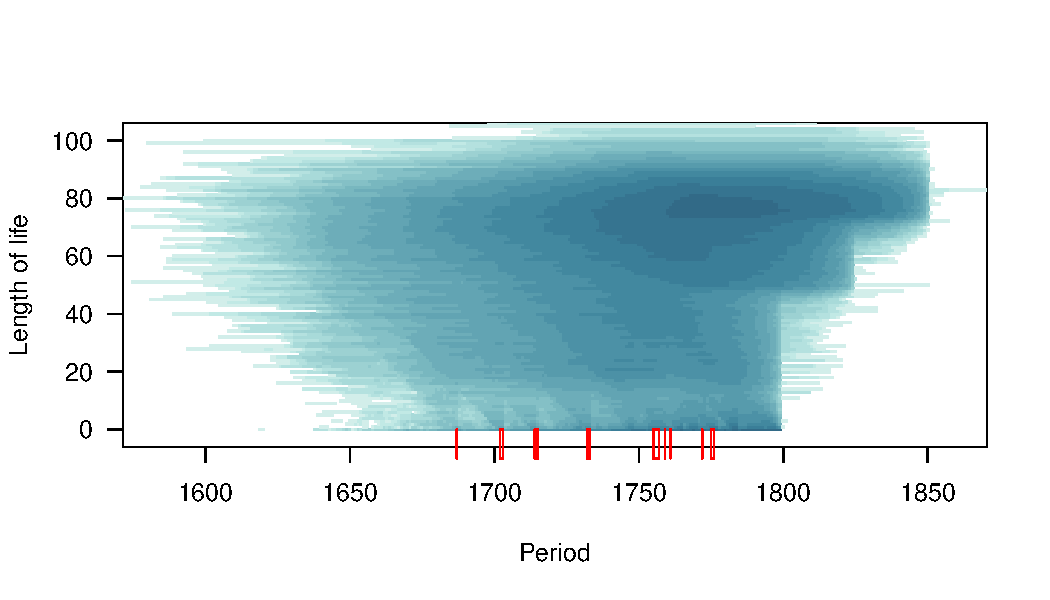
\includegraphics[scale=.9]{Figures/QuebecLP.pdf}
\caption{Population structure by length of life and year. Logged counts}
\label{fig:lpq}
\end{figure}

\begin{small}
%In this orientation,  
%It would appear births were not collected after 1800, and some other data
% collection milestone happens in 1825. 
%The triangles at the bottom look like artifacts at first, but actually they are
% mortality shocks (wow!). Take a given triangle: each is right-aligned on moment of death (otherwise a given lifeline would be higher up in y and extend further to the right in x). These shocks likely extend up into higher ages, but they get blurred out by higher baseline mortality in higher ages. I guess growth happens in the contours for the most part because the population was growing exponentially.

%What are the boundaries on the extreme right, and why do some lifelines extend
%beyond the main boundaries?  In addition, if you look at the triangle with
% right vertical axis in 1705 or so, and left oblique edge of slope -1 extending upward
%and to the left at 45$^\circ$ from horizontal axis, that oblique image seems to
%extend very far up, detectably as far up as life length 70.  There is a
% parallel shift in density to the left of that oblique line space by about 10-15 years.  I am wondering if we are looking at an artifact of some kind of grouping of the data or if there really was a crisis in mortality around 1690, 1705, 1720, 1740, 1750, …  If you have independent estimates of death rates in these years, it would probably be easy to compare those estimates with these apparent events.

Death info here comes from burial records, which had some age constraints in
data collection: (1800-1825:deaths of 50+ only; 1826-1850: deaths of 75+ only).
That explains the block edges on the right of LP, and the angle edges in TC. I'm
also not very sure what accounts for the exceptions to these edges, but my guess would be that it owes to there being multiple potential sources for date of death. Here it is again, with known epidemics (i.e. main disease can be guessed) marked with red rectangles (if spanning more than 1 year)
\citep[cf Figure 1.1][]{mazan2011}Typhus, measles, smallpox, etc) were cross
checked with other historical documents. These match the right edge of most of the triangles, and the others may have just been lesser or unstudied epidemics, or ones that I just missed. The left oblique edge of each triangle is in general more visible than the vertical right edge, at least in the early part of the series, because growth in the early phase (pre 1663 if I recall) was largely from migration.

Missingness in LP:
Data collection began in 1621, but lifelines in the LP figure begin well left of that. This is because a person dying at some old age right at the start of the series will have of course been born well before the series itself began. Anything to the left of 1621 is incomplete in a sense, because we're missing the lifetlines that would overlap the pre 1621 lives we already have (e.g. a life extinguished at age 50 in 1620). So, we could of course crop the surface at 1621, no problem. However, we have the same problem on the right side of the series. Ignoring the block shapes for now.  A person dying in 1850 at age 60 would clearly overlap with part of the blue we have, but would here be excluded. The right-side zone of still-incomplete observation in LP is the upper-right triangle of the whole surface; so, draw a line inward from the lower right corner at slope -1. Anything above that is still missing the early part of some lives. Those funny observation blocks offset said missingness to some degree, a happy accident. As a rule, missingness is higher in LP as we go up the y axis on the right side.

Now imagine we have an LP surface of the prevalence pi(l,p) of some health condition from HRS. The observation window is much smaller, but we are located high up in the lifespan range. Most of the people whose prevalence should contribute to  pi(90,2015) have not died yet, because many of them are still toddlers. Others not yet included in  pi(90,2015) are those age 80 in 2015 that will not die until 2025. None of this will be a problem if we condition these planes on some other bounding time measure, I guess it's just something to be careful with. My first guess as to conditions that might vary in a regular way over LP would be prevalence of having ever smoked. Here's a screenshot of the TAL plane of the 1915 female birth cohort for ever-smoking prevalence:

I used this as an example in another recent paper (link). I found this striking.
 Lifespan contours are those with slope -1. One explanation would be that smoking determines length of life before age 70 and things simply don't change thereafter (you can't undo being an ever smoker). As I recall dental visits had contours with this slope, but the surface was not monotonic. It's just a guess that strong patterns like these would carry over into LP.

The Quebec data has an incredible observation window, but no health except fertility (and extended family events). Lifeline surfaces like those produced for Quebec can be inferred from any Lexis surface of death counts.
\end{small}

\subsection{TC}

The thanatological age distribution of a birth cohort specifies that birth
cohort's life table (distribution of T given C). Conversely, the distribution of
birth cohorts of people of a given thanatological age reveals mortality history and inequalities in
survival. If more of the people who will die in 5 years are from recent cohorts
than from cohorts long ago, this population has high childhood mortality and low survival to old ages.

A lifeline on the CT plane extends from 0 upward until the age of death. Ergo,
someone born in 1700 dying at age 80 contributes 1 to the count in each thanatological age from 0 to 80, the entire countdown. T = 0 is maximally heterogenous with respect to A (or L or D or P), and lifeline overlap decreases in higher T (long-lived people while they're young, i.e. in years closer to C itself). Here's that tabulation of this same data (also logged):

\begin{figure}
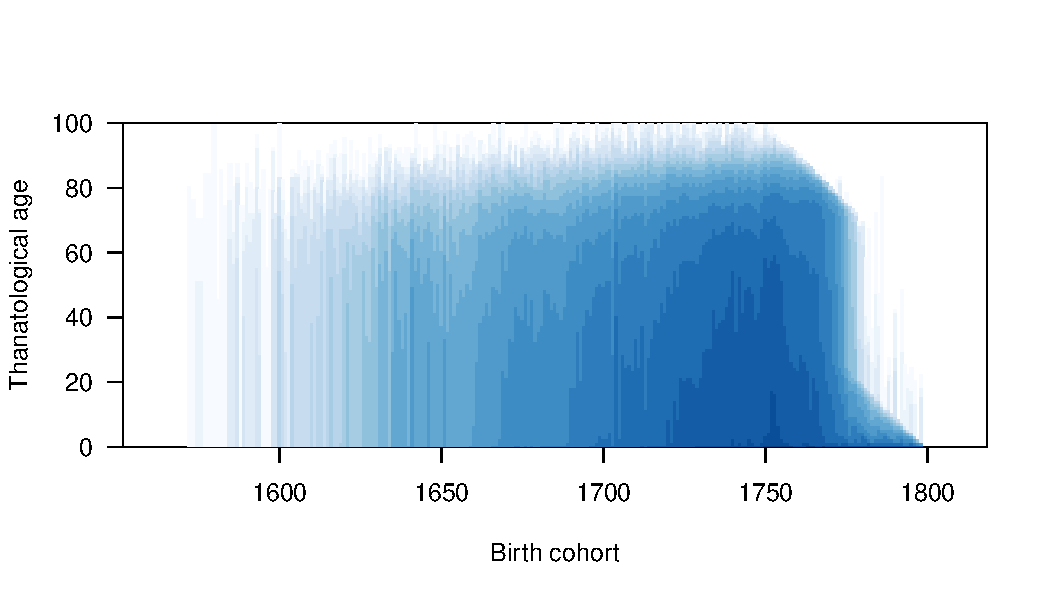
\includegraphics[scale=.9]{Figures/QuebecTC.pdf}
\caption{Population structure by time to death and birth cohort.}
\label{fig:tcq}
\end{figure}

The first thing to pop out at me are birth dearths for particular years,
possibly the same years that were the right edges of mortality shocks in the LP surface. Also a wider boom or two, which might just be natural growth. Here each vertical strip monotonically decreases as we go up to higher thanatological ages. I agree these are the stationary populations belonging to each birth cohort, each with a radix equal to the actual birth cohort size, so this is a bit more straightforward to wrap one's mind around than LP.

It seems that the upper envelope (that is, the thanatological
age at which the lifelines terminate, as a function of cohort) is rising with increasing cohort, reflecting improvements in cohort life expectancy.  These improvements are visible also in contour lines that are lower than the upper envelope.  You suggested that growth happens in the contours mainly because the population was growing exponentially.  If you wanted to remove the effect of population growth, you could plot a curve of births or a curve of population size or a curve of number of women in the population below the x axis with an inverted y axis and then normalize the counts by births or population size or number of women.  That might reveal additional patterns.  This kind of normalization by some measure of population size might also be applied to the next figure.

​I now detect the affects of the right-side block observation of deaths. Had burial records for younger ages been captured in this data, we would have increasing contours as we go down towards the x axis on the right side. Here we just get the tips of the oldest deaths, each having needed to pass through young ages first, so they trace down to age 0.​

\subsection{AD}

For a given age A, the distribution of the death cohort D of individuals gives
the conditional life table, conditional on reaching the given age A, and hence gives, for example, the remaining life
expectancy and the variability of remaining life, among other summaries of the
conditional life table. Conversely, for a given death cohort D, the distribution
of age A of individuals specifies the distribution of their birth cohorts and life lengths.

\begin{figure}
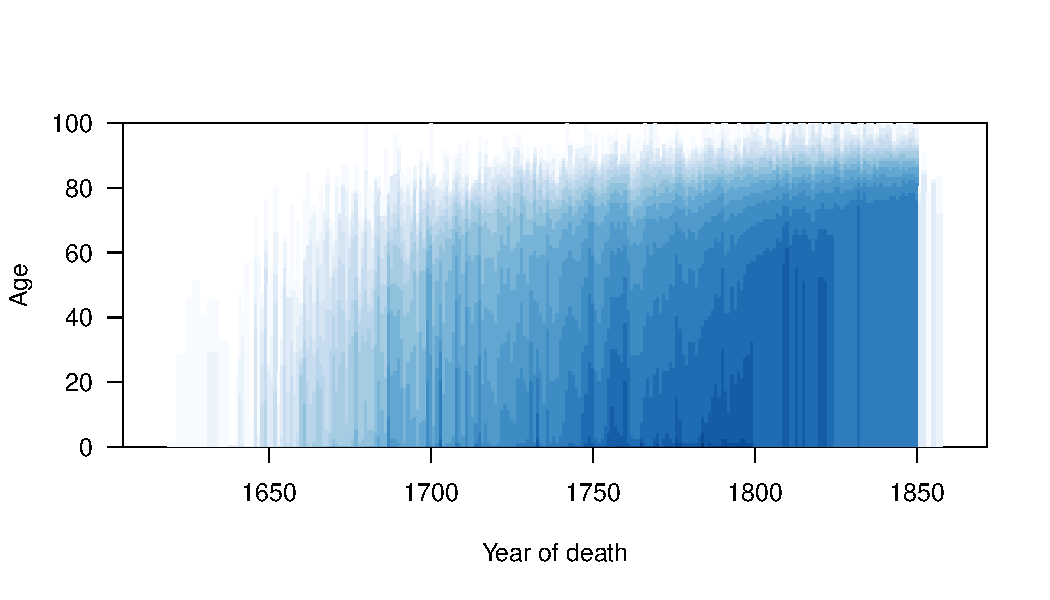
\includegraphics[scale=.9]{Figures/QuebecAD.pdf}
\caption{Population structure by age and year of death.}
\label{fig:adq}
\end{figure}
In the AD plane, we have the same sort of vertical overlap. Just as everyone
experiences T = 0, everyone is also included in A = 0 here. If this were a stationary population then a vertical strip here would be equal to one from the CT plane, but we have lots of non-stationary things happening. Vertical striation here is due to mortality shocks in particular years, and these are strictly positive. Anything dearthy-looking is either due to a 'harvest' or data collection oddities. At least I've never heard of a survival shock. So, to repeat, an individual born in 1700 destined to die at age 80 is located at 1780 in the x axes, and ages from the bottom up. Ergo, the bottom of the surface is young people, as we're used to, but they come from different birth cohorts. As with CT, the population is maximally mixed with respect to C (or L or P or T) at A = 0. An 80 year old and an infant dying in 1780 both contribute to the count at age 0 in 1780.

We see here the same high density in death year 1705 that we detected in the LP
plane, so maybe it is not a data artifact. Whether there are also high densities of deaths in the other years we identified in the LP plane is not so clear to me; perhaps yes. There appear to be little white rectangles between 1760 and 1800 at ages zero through perhaps 3 or 4. Every lifeline must extend to age zero, so something is wrong here, I think. Again we see the upper envelope increasing with the year of death and rising contour lines.

\section{Independant time surfaces as cross-sections}
Here use example of HRS surfaces produced at novel \emph{cut} angles.
\subsection{LP}

\subsection{TC}


\subsection{AD}

% bibliography
\bibliographystyle{chicago}
\bibliography{references}  
\end{document}

